\section{eo\-Elite\-Sequential\-Select$<$ EOT $>$ Class Template Reference}
\label{classeo_elite_sequential_select}\index{eoEliteSequentialSelect@{eoEliteSequentialSelect}}
All Individuals in order.  


{\tt \#include $<$eo\-Sequential\-Select.h$>$}

Inheritance diagram for eo\-Elite\-Sequential\-Select$<$ EOT $>$::\begin{figure}[H]
\begin{center}
\leavevmode
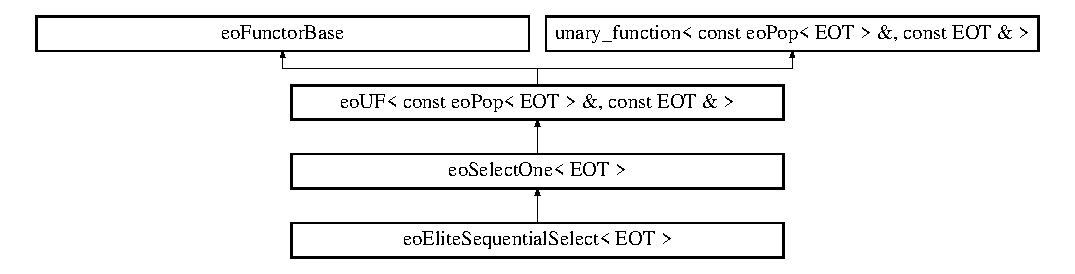
\includegraphics[height=3.23699cm]{classeo_elite_sequential_select}
\end{center}
\end{figure}
\subsection*{Public Member Functions}
\begin{CompactItemize}
\item 
{\bf eo\-Elite\-Sequential\-Select} ()\label{classeo_elite_sequential_select_a0}

\begin{CompactList}\small\item\em Ctor: sets the current pter to numeric\_\-limits$<$unsigned$>$::max() so init will take place first time not very elegant, maybe ... \item\end{CompactList}\item 
void {\bf setup} (const {\bf eo\-Pop}$<$ {\bf EOT} $>$ \&\_\-pop)\label{classeo_elite_sequential_select_a1}

\begin{CompactList}\small\item\em virtual function to setup some population stats (for instance eo\-Proportional can benefit greatly from this) \item\end{CompactList}\item 
virtual const {\bf EOT} \& {\bf operator()} (const {\bf eo\-Pop}$<$ {\bf EOT} $>$ \&\_\-pop)\label{classeo_elite_sequential_select_a2}

\begin{CompactList}\small\item\em The pure virtual function that needs to be implemented by the subclass. \item\end{CompactList}\end{CompactItemize}
\subsection*{Private Attributes}
\begin{CompactItemize}
\item 
unsigned {\bf current}\label{classeo_elite_sequential_select_r0}

\item 
std::vector$<$ const {\bf EOT} $\ast$ $>$ {\bf eo\-Pters}\label{classeo_elite_sequential_select_r1}

\end{CompactItemize}


\subsection{Detailed Description}
\subsubsection*{template$<$class EOT$>$ class eo\-Elite\-Sequential\-Select$<$ EOT $>$}

All Individuals in order. 

The best individual first, then the others in sequence (random order). for G3 evolution engine, see Deb, Anad and Joshi, CEC 2002

As {\bf eo\-Sequential\-Select}{\rm (p.\,\pageref{classeo_sequential_select})}, it is an {\bf eo\-Select\-One}{\rm (p.\,\pageref{classeo_select_one})} to be used within the eo\-Easey\-EA algo, but conceptually it should be a global {\bf eo\-Select}{\rm (p.\,\pageref{classeo_select})}, as it selects a bunch of guys in one go (done in the setup function now) 



Definition at line 97 of file eo\-Sequential\-Select.h.

The documentation for this class was generated from the following file:\begin{CompactItemize}
\item 
eo\-Sequential\-Select.h\end{CompactItemize}
